\documentclass[12pt, a4paper]{elsarticle}

% ---- Packages ----
\usepackage{graphicx}
\usepackage{amsmath}
\usepackage{amssymb}
\usepackage{booktabs}
\usepackage{multirow}
\usepackage{microtype}
\usepackage{lmodern}
\usepackage[T1]{fontenc}
\usepackage[utf8]{inputenc}
\usepackage{setspace}
\usepackage{hyperref}
\usepackage{lineno}

\journal{Journal of Biomechanics}
\biboptions{authoryear}

\begin{document}
\onehalfspacing
\linenumbers

\begin{frontmatter}

\title{A Two-Step Weighted Inverse Kinematics Framework to Improve Biological Validity in Kinematic Modelling of Post-Stroke Upper Limb Motion}

\author[hw]{Abdul Maajid Aga\corref{cor1}}
\ead{abdulmaajidaga@outlook.com}
\author[hw]{Shawgi Mounis}

\cortext[cor1]{Corresponding Author}
\address[hw]{Department of Engineering and Physical Sciences, Heriot-Watt University Dubai Campus, Dubai Knowledge Park, PO Box 501745, Dubai, United Arab Emirates}

\begin{abstract}
Sparse optical marker sets are practical for clinical stroke assessments, but standard inverse kinematics (IK) fails on these data due to spatial mismatch and kinematic redundancy. Computational models assume fixed anatomical geometries, so mapping chest markers from patients of varying body proportions creates a moment-arm mismatch that causes Standard IK solvers to collapse numerically (mean errors $>$300 mm). We propose a Two-Step Weighted IK framework to resolve this. First, trunk lean is derived from the geometric orientation of chest markers via Singular Value Decomposition (SVD), yielding a rotation angle unaffected by differences in chest depth. Second, with the trunk fixed, arm kinematics are recovered using a two-tier weighted Jacobian that prioritises arm joints over the shoulder girdle. Evaluated on 24 stroke survivors with severe hemiparesis and 49 healthy controls, the pipeline stabilised the solver, reducing mean reconstruction errors by approximately 85\% compared to standard models (from $>$300 mm down to 44.97 mm for stroke and 39.47 mm for healthy subjects). Crucially, the method recovered expected clinical biomarkers that standard solvers completely obscure: it successfully quantified compensatory trunk forward lean (4.3° stroke vs.\ 3.1° healthy), and accurately captured the flexor-synergy pronation gap ($+$7.7°) and blunted shoulder elevation ($-$9.1°) in alignment with established post-stroke physiological trends. Two solver-independent metrics (wrist reach distance and reach-path-ratio) confirm that these separations reflect genuine physiological impairment. The framework enables reliable extraction of pathological kinematics from standard clinical motion-capture data.
\end{abstract}

\begin{highlights}
\item Tracking trunk position fails due to severe model-to-patient depth mismatches.
\item Standard inverse kinematics fails on sparse markers, causing errors over 300mm.
\item Step one computes trunk lean via geometric orientation to fix depth scaling errors.
\item Step two applies biological penalty weights to prevent false shoulder exploitation.
\item Accurately captures true stroke traits: trunk lean, synergy, and shoulder limits.
\end{highlights}

\begin{keyword}
inverse kinematics \sep musculoskeletal modelling \sep compensatory strategies \sep trunk kinematics \sep upper extremity biomechanics
\end{keyword}

\end{frontmatter}

% ================================================================
\section{Introduction}
\label{sec:intro}

Capturing accurate upper-limb kinematics in a routine clinical setting presents a significant methodological challenge, yet it is essential for evaluating rehabilitation outcomes. Dense, full-body optical marker sets are largely impractical for routine clinical use. While sparse marker sets are accessible, they introduce severe challenges in computational modelling. Standard inverse kinematics (IK) solvers, such as those embedded in OpenSim \cite{delp2007} or MuJoCo \cite{todorov2012}, optimise purely for global spatial accuracy and treat all degrees of freedom (DOFs) equally. When applied to sparse clinical marker sets, this uniform weighting amplifies model uncertainty and produces anatomically false joint angles \cite{uchida2022}. A primary failure point is tracking the trunk by following the absolute position of chest markers: human chest depth varies considerably between individuals, but computational models have a fixed skeletal depth. This geometric mismatch means the same marker movement maps to different joint angles depending on the patient's body shape, making Standard IK numerically unstable and causing large reconstruction errors.

Deriving appropriate kinematics is even more difficult in post-stroke rehabilitation because patients actively compensate for impairments using other body parts. A primary clinical objective is identifying and quantifying these exact compensatory motor strategies. For example, Cirstea and Levin demonstrated that patients recruit compensatory forward trunk flexion to augment their functional reaching range when shoulder and elbow mobility are impaired \cite{cirstea2000, jayasinghe2021}. McPherson and Dewald documented the abnormal flexor synergy, a stereotyped coupling that links elbow flexion to forearm pronation and shoulder abduction \cite{mcpherson2022}. Furthermore, stroke results in elevated sternoclavicular joint excursion \cite{mccrea2005, michaelsen2001} alongside a general reduction in the shoulder elevation arc \cite{choi2023}. Because standard IK suffers from the chest-depth scaling mismatch, the solver artificially activates the shoulder girdle to absorb residual tracking errors. Consequently, standard methods fail to properly estimate these movements; they destroy the exact stroke-specific compensatory signals clinicians need to track, replacing genuine pathological biomarkers with solver artefacts.

We address these methodological limitations by introducing a Two-Step Weighted IK framework. By relying on geometric orientation rather than spatial translation for the trunk, we extract a biologically accurate lean that is immune to scaling errors. We pair this with a 2-tier biologically weighted Jacobian solver for the arm, which naturally isolates genuine pathological movement from sparse clinical data. Section~\ref{sec:methods} details the framework design; Section~\ref{sec:results} presents reconstruction and clinical metric results; Section~\ref{sec:discussion} situates the findings in the context of clinical biomechanics.

% ================================================================
\section{Methods}
\label{sec:methods}

\subsection{Participants and Dataset}
Data were drawn from the MHH U-Limb motion capture dataset \cite{averta2021ulimb}. To ensure a uniform and homogenous cohort, the dataset was filtered to include only right-hand-affected stroke patients and right-hand-dominant healthy controls. Quality screening excluded Subject 01 (the medial epicondyle marker was missing in 22–31\% of frames across all trials, corrupting the elbow joint-centre estimate) and recording 15\_12\_1 (complete medial epicondyle marker absence). The analytic cohort comprised 73 participants: 24 individuals with chronic unilateral stroke (Fugl-Meyer Assessment scores 16–20, indicating severe upper-limb impairment \cite{woodbury2013}; mean $\approx$ 18.6) and 49 healthy controls.

Participants performed a standardised sagittal drinking task: reaching forward to grasp a cup, lifting it to the mouth, and returning it. Kinematics were recorded at 200 Hz using a passive optical system. Before inverse kinematics, the raw markers were mapped to five model inputs, each serving a distinct role. Four were used as IK targets: \texttt{V\_Shoulder} (placed at the acromion), \texttt{V\_Elbow} (midpoint of the medial and lateral epicondyle markers, estimating the elbow joint centre), \texttt{V\_Wrist} (mean of the medial and lateral wrist markers, estimating the wrist joint centre), and \texttt{V\_Vector} (the axis defined by two wrist markers, encoding forearm pronation/supination). The fifth input, a four-marker rigid chest plate cluster (\texttt{CS\_1}–\texttt{CS\_4}) placed on the upper sternum, was used solely to estimate trunk orientation via SVD plate-normal decomposition (Section~\ref{sec:weighted}) and was not passed to the IK solver as a positional target.

\subsection{Model Geometry and Segment-Aware Preprocessing}
We utilised the MyoSuite arm model (\texttt{myoarm.xml}) \cite{caggiano2022}. To capture compensatory body movement, we extended the base model by adding a sagittal \texttt{trunk\_forward\_lean} joint (rotation axis aligned to the coronal plane), producing \texttt{myoarm\_trunk.xml}. The base MyoSuite model contains several mathematical correction joints (\texttt{unrotscap}, \texttt{acromioclavicular}, \texttt{unrothum} variants, and \texttt{shoulder1\_r2}) that implement internal kinematic constraints rather than physiological DOFs. All nine correction joints were fixed at zero throughout. This stops the solver from moving them to reduce error, which would otherwise produce anatomically impossible poses.

Standard scaling applies a single arm-length ratio to the whole body. This fails when a subject has long arms but a narrow torso, projecting chest markers at the wrong location. We therefore implemented \textit{segment-aware scaling}: arm markers were scaled via a \texttt{model\_arm / lab\_arm} ratio, while chest markers were scaled independently using a \texttt{model\_shoulder\_to\_CS / lab\_shoulder\_to\_CS} ratio. These two factors differed by 10–15\% within individual subjects. A rigid-body rotation \cite{wahba1965} was then applied to align the lab's shoulder-to-elbow axis with the model's resting orientation.

\subsection{Prior Trunk Approaches and Their Failure Modes}
\label{sec:prior_trunk}
Before arriving at the SVD prescription, three approaches to recovering trunk angle were evaluated and rejected.

\textbf{Standard IK: free trunk behaviour.} Leaving \texttt{trunk\_forward\_lean} as an unconstrained DOF with uniform low damping allows the solver to move it freely. Because the arm markers are defined relative to the shoulder, they carry almost no sensitivity to trunk movement in the Jacobian. The solver therefore sets trunk angles to absorb leftover arm residuals rather than tracking actual trunk movement. Empirical evaluation across six representative trials revealed that the resulting trunk angles were actively anti-correlated with the CS plate ground truth ($r = -0.689$, $p = 0.130$), meaning the solver moves the trunk in the opposite direction to actual patient lean.

\textbf{Heavy trunk damping (neutral-start).} Assigning a large regularisation weight to the trunk DOF and initialising it at 0° suppresses trunk motion unless arm residuals are very large. Low damping ($w = 0.05$) yielded $r = -0.864$ ($p = 0.026$) and heavy damping ($w = 50.0$) yielded $r = -0.874$ ($p = 0.023$) against the CS plate ground truth; both results were significantly anti-correlated, and increasing the penalty worsened the correlation rather than improving it. A sweep over five weights ($w \in \{0.5, 1.0, 5.0, 10.0, 50.0\}$) confirmed this, with $r$ ranging from $-0.07$ to $-0.87$; the damping value does not change the direction of failure.

\textbf{CS markers with delta motion.} Including the chest cluster as direct IK positional targets addresses the problem geometrically. A depth mismatch remains: the model's chest is fixed at $\sim$320 mm depth, while actual chest depths in our cohort ranged from 82 to 374 mm (SD = 137 mm). Applying \textit{delta motion} (frame-by-frame displacement from a frame-zero baseline rather than absolute position) removes the static offset. However, it cannot remove the depth-dependent scaling of rotations: the same 5° trunk lean produces a different marker displacement in a shallow-chested versus a deep-chested subject. The same delta therefore maps to different joint angles in different subjects, making position-based trunk IK fundamentally unreliable across individuals.

All three approaches confirm that IK cannot recover trunk angle from marker positions, and that naive attempts produce actively misleading results. This motivated the orientation-based approach described below.

\subsection{Primary Contribution: Two-Step Weighted IK}
\label{sec:weighted}
To bypass the geometric distortion of chest markers and stabilise the solver, we implemented a Two-Step Weighted IK framework.

\textbf{Step 1: Geometric Trunk Prescription (SVD).} 
To avoid the depth mismatch described in Section~\ref{sec:prior_trunk}, we measure orientation rather than position. We compute the SVD of the four-marker chest plate (CS\_1–CS\_4), and the resulting plate normal gives the forward lean angle directly. Because orientation does not depend on chest depth, this angle is consistent regardless of body size. It is prescribed directly to the \texttt{trunk\_forward\_lean} DOF, locking the trunk to the patient's actual posture.

\textbf{Step 2: 2-Tier Weighted Jacobian Arm IK.}
With the trunk fixed, the remaining upper limb DOFs are recovered using a regularized damped least-squares IK solver:
\begin{equation}
\label{eq:dls}
dq = (J^T J + W)^{-1} J^T e
\end{equation}
Standard IK uses a uniform matrix for $W$, causing redundancy exploitation. We replace this with a 2-tier diagonal damping matrix grounded in the force-reserve principle, whereby the central nervous system (CNS) preferentially recruits motor commands that preserve a margin below maximum effort \cite{faity2024}, combined with the weighted Jacobian formulation \cite{khoramshahi2022} (Table \ref{tab:damping_hierarchy}):

\begin{enumerate}
    \item \textbf{Tier 1 (Arm):} The 7 primary arm effectors (deviation, flexion, pro/sup, elbow\_flexion, elv\_angle, shoulder\_elv, shoulder\_rot) are assigned a cheap baseline damping of $w=0.05$.
    \item \textbf{Tier 2 (Sternoclavicular (SC) Girdle):} The scapular protraction and elevation joints are assigned a penalty weight of $w=0.20$ (a 4× penalty), ensuring the solver exhausts arm mobility before shrugging the shoulder girdle.
\end{enumerate}

\begin{table}[htbp]
  \centering
  \caption{Two-Tier Damping Hierarchy Summary. The biological cost matrix designed to mimic the CNS force-reserve hierarchy.}
  \label{tab:damping_hierarchy}
  \vspace{0.5em}
  \resizebox{\linewidth}{!}{%
  \begin{tabular}{llccp{2.5cm}}
    \toprule
    \textbf{Group} & \textbf{DOFs} & \textbf{Damp} & \textbf{Ratio} & \textbf{Rationale} \\
    \midrule
    Arm & wrist, elbow, shoulder (7) & 0.05 & 1× & Primary effectors. \\
    SC Girdle & sternoclavicular\_r2/r3 & 0.20 & 4× & Proximal penalty. \\
    \bottomrule
  \end{tabular}}
\end{table}


The Tier 2 SC penalty of 0.20 was empirically validated across the full cohort of 73 trials (24 stroke, 49 healthy). Compared to uniform damping ($w=0.05$), the hierarchy reduced mean IK reconstruction error from $44.97 \pm 27.34$ mm to $38.69 \pm 21.96$ mm and suppressed peak sternoclavicular excursion from $0.95 \pm 1.91$° to $0.14 \pm 0.51$°; both effects were statistically significant (Wilcoxon signed-rank, $p < 0.001$; Figure \ref{fig:damping_comparison}). Finally, the trunk was initialised at 0° for the first frame to prevent the solver settling on a false resting posture; it was released to the weighting hierarchy for all remaining frames.

\begin{figure}[!t]
    \centering
    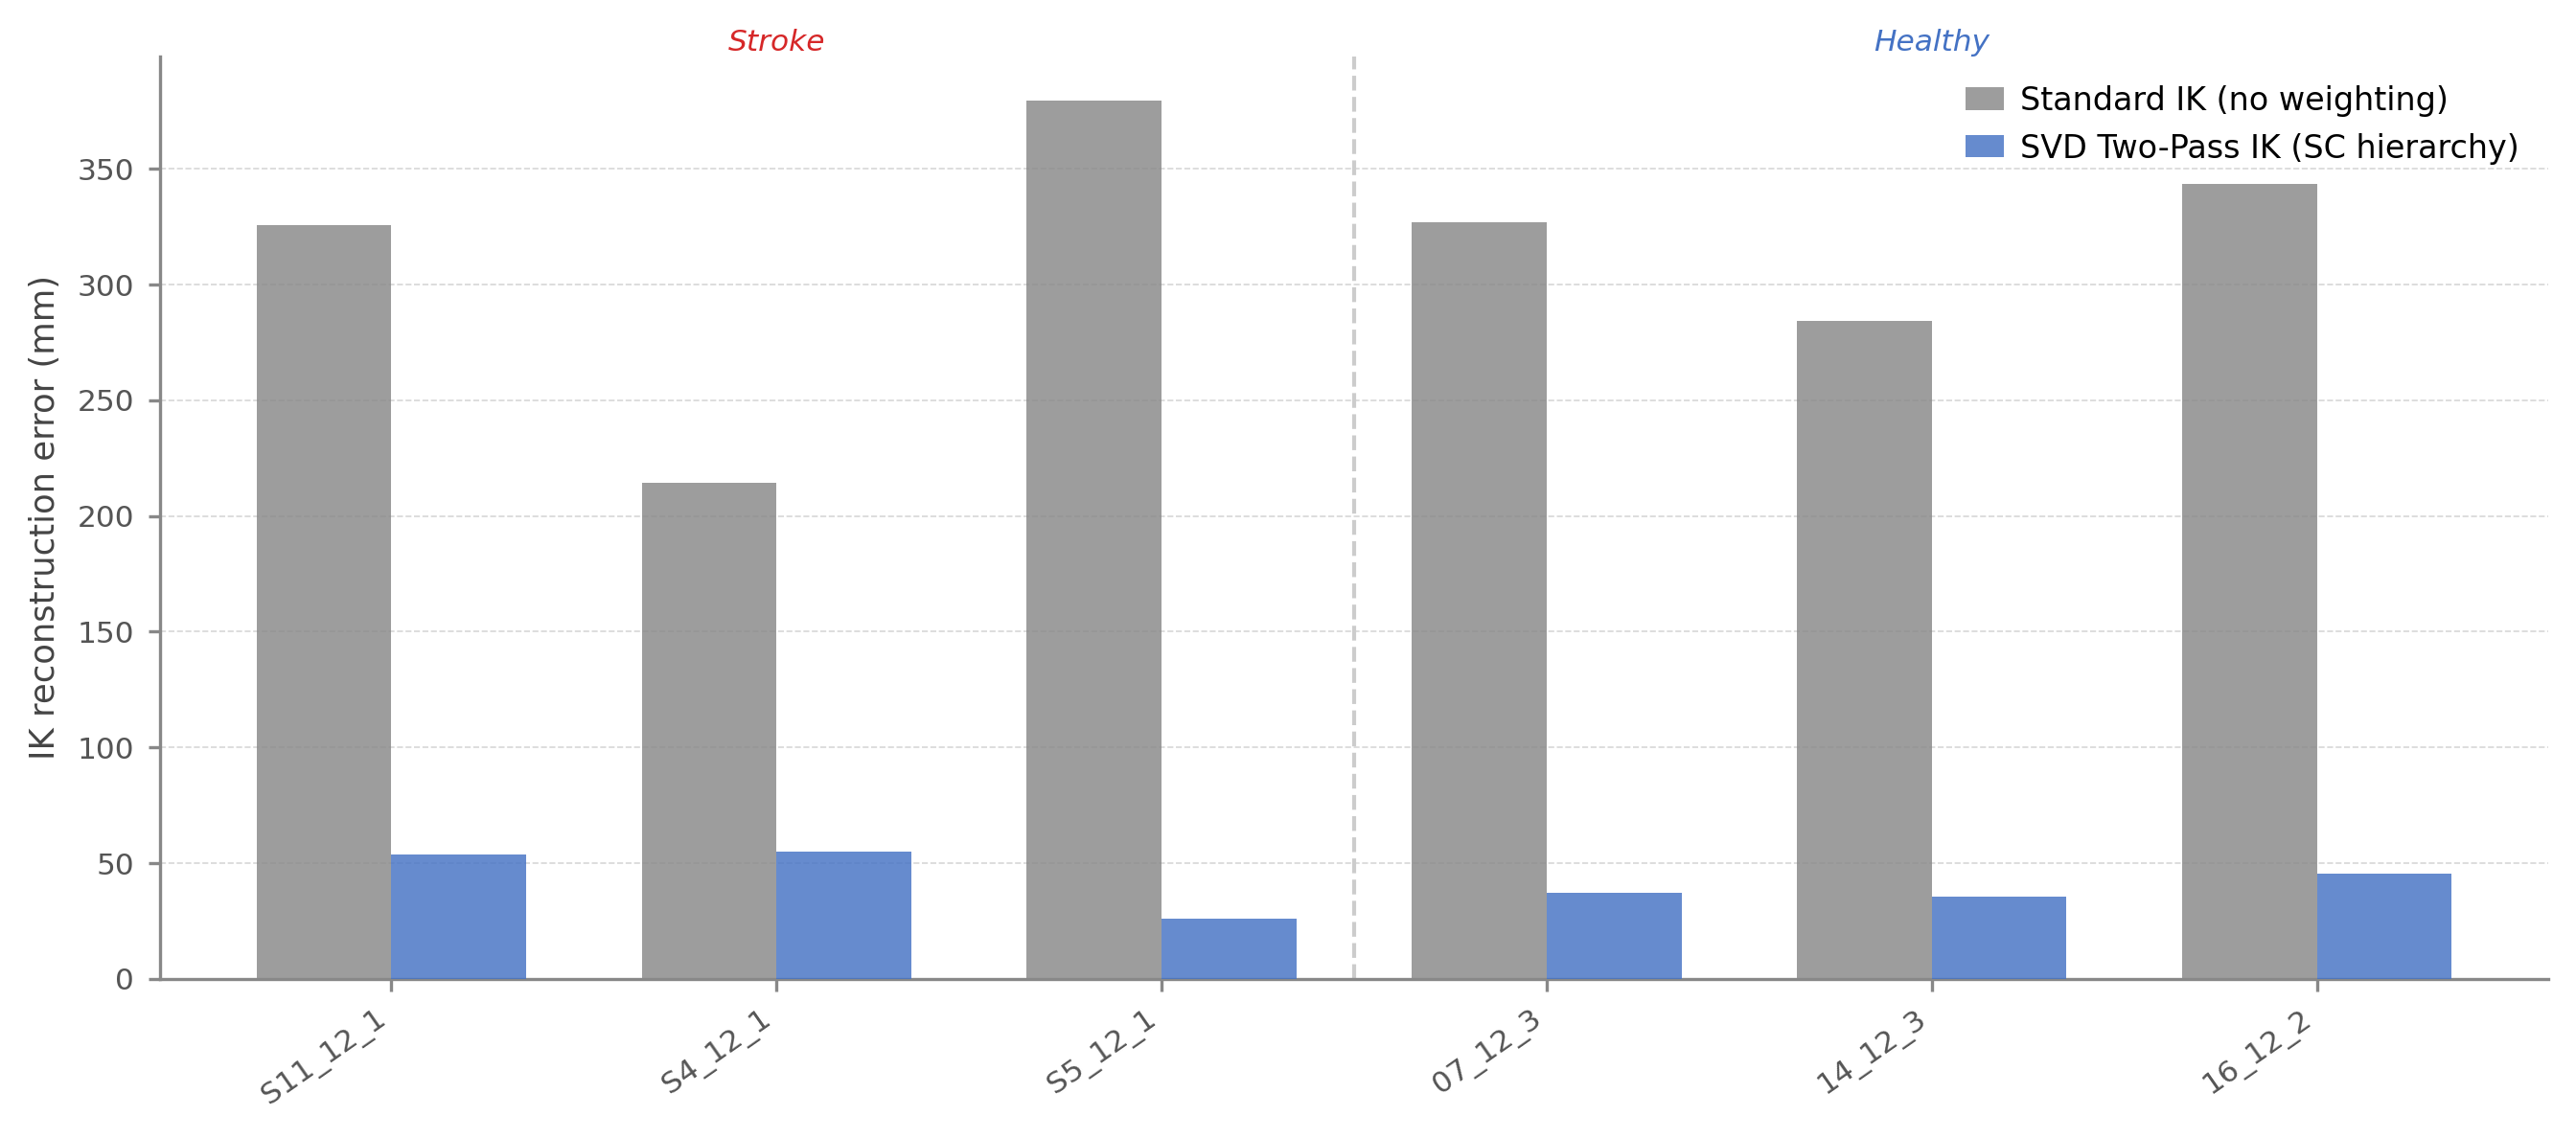
\includegraphics[width=\linewidth]{damping_comparison.png}
    \caption{SC damping hierarchy validation across 73 trials. SC=0.20 reduces IK reconstruction error and suppresses spurious sternoclavicular excursion relative to uniform damping (SC=0.05; Wilcoxon $p < 0.001$).}
    \label{fig:damping_comparison}
\end{figure}

\subsection{Pipeline Verification}
\label{sec:pipeline_verification}
To confirm that the SVD-prescribed trunk angles are internally consistent, a pipeline verification check was performed. The SVD-derived orientation was compared against raw chest marker coordinates across 70 trials, yielding $r = 0.977$ (Figure \ref{fig:ik_vs_cs_correlation}). This confirms that the orientation-based approach captures the chest plate's true sagittal movement without introducing numerical artefacts.

\begin{figure}[!t]
    \centering
    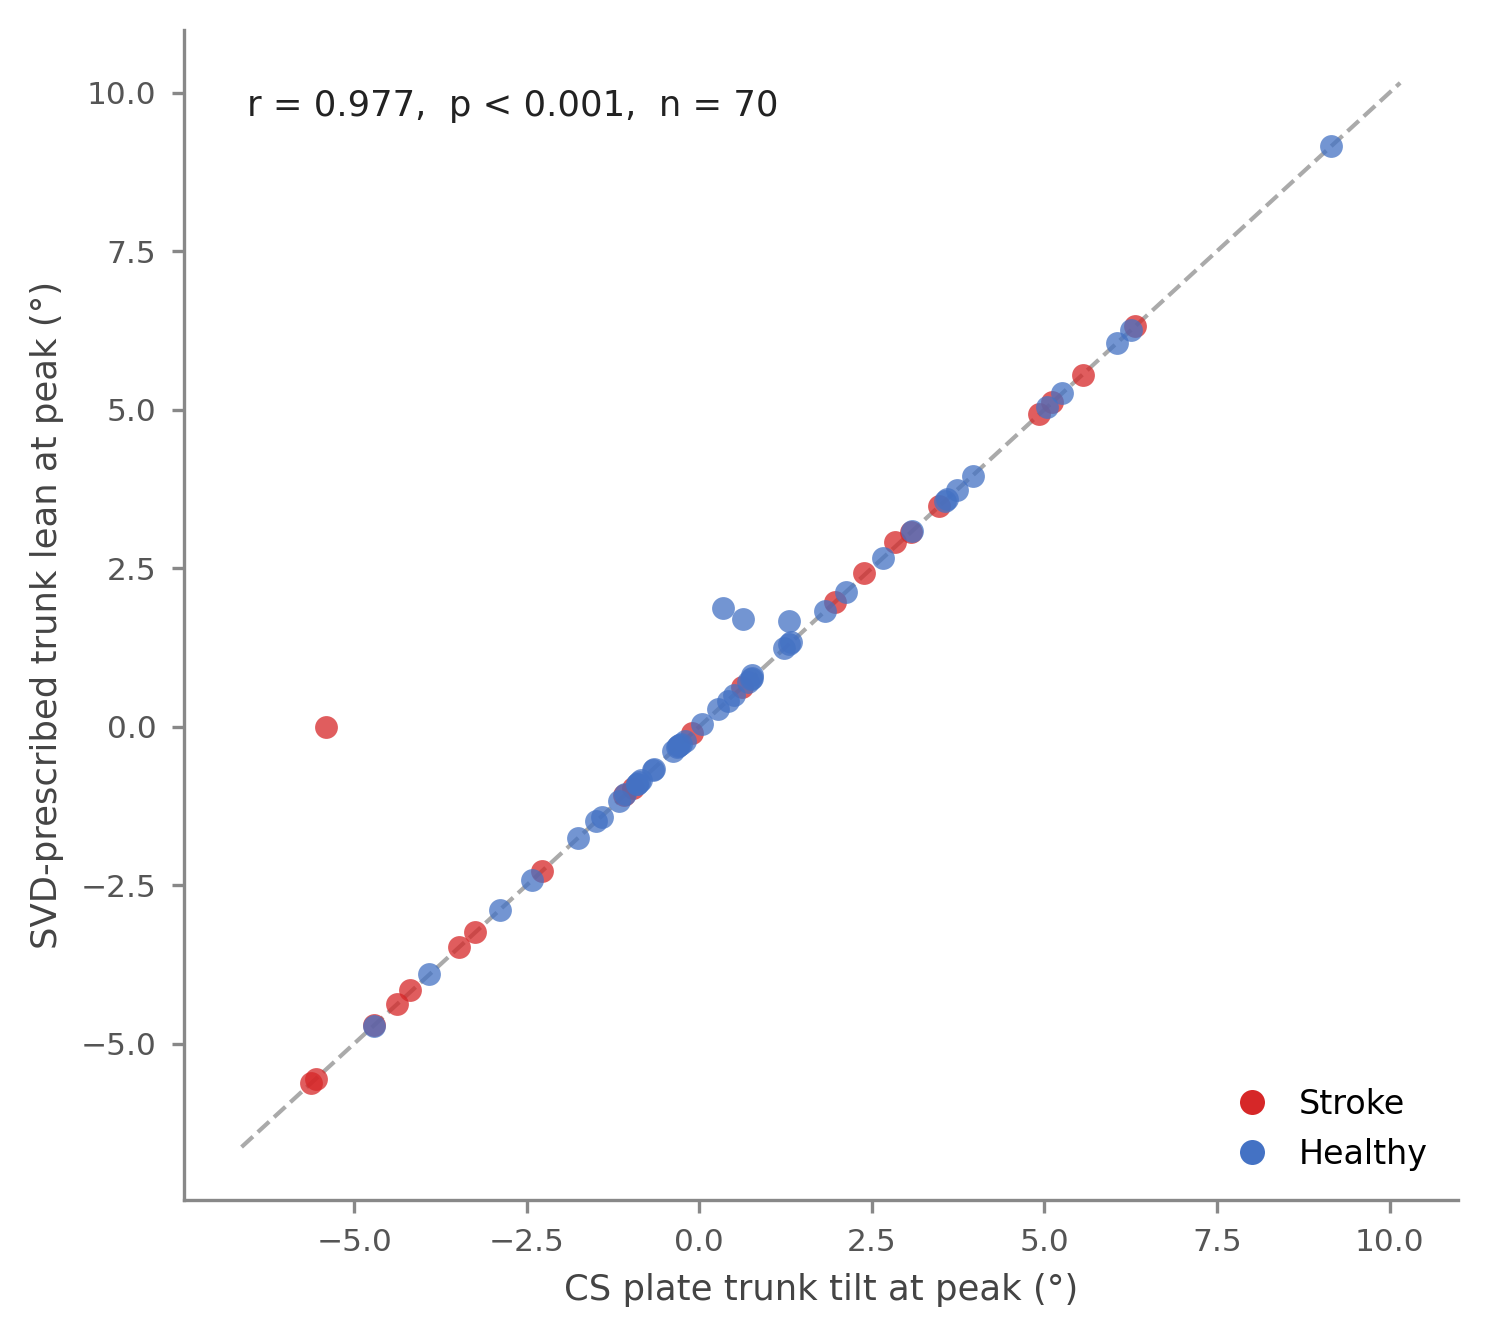
\includegraphics[width=\linewidth]{ik_vs_cs_correlation.png}
    \caption{Pipeline verification scatter plot ($n = 70$ trials after outlier filtering). x-axis: trunk tilt derived from the CS chest plate SVD normal (degrees); y-axis: \texttt{trunk\_forward\_lean} prescribed by the IK pipeline (degrees). Pearson $r = 0.977$, $p < 0.001$, confirming that the SVD-prescribed trunk angles track the geometric plate normal consistently across the full cohort.}
    \label{fig:ik_vs_cs_correlation}
\end{figure}

\subsection{Evaluation Metrics}
Six clinical metrics were tracked. Solver-independent metrics (Wrist Reach Distance and Reach-Path-Ratio) were computed from raw 3D marker coordinates to confirm baseline impairment without relying on the solver. IK-dependent metrics (Trunk Forward Lean, Forearm Pronation, Shoulder Elevation, Elbow ROM) were extracted from the joint angle output to assess the solver's clinical validity.

% ================================================================
\section{Results}
\label{sec:results}

\subsection{IK Reconstruction Error}
The implementation of the Two-Step Weighted IK pipeline dramatically improved marker reconstruction accuracy (Table \ref{tab:reconstruction_error}). Standard IK was numerically unstable due to the moment arm mismatch. With the trunk having near-zero influence on shoulder-relative markers, the solver assigned arbitrary trunk values to reduce arm residuals rather than tracking genuine trunk movement. This produced mean reconstruction errors of 306.53 $\pm$ 84.20 mm (Stroke) and 318.22 $\pm$ 30.64 mm (Healthy). By prescribing the trunk geometrically via SVD and applying the 2-Tier biological cost matrix to the arms, the system stabilised completely, dropping errors to 44.97 $\pm$ 16.28 mm (Stroke) and 39.47 $\pm$ 5.35 mm (Healthy), representing a 6.8-fold reduction (306 mm $\rightarrow$ 45 mm). This confirms that resolving geometric mismatch and applying biological cost constraints are both necessary conditions for solver stability on sparse clinical marker sets.

\begin{table}[htbp]
  \centering
  \caption{IK Reconstruction Error (Mean $\pm$ SD per subject).}
  \label{tab:reconstruction_error}
  \vspace{0.5em}
  \resizebox{\linewidth}{!}{%
  \begin{tabular}{lcc}
    \toprule
    \textbf{Method} & \textbf{Stroke (mm)} & \textbf{Healthy (mm)} \\
    \midrule
    Standard IK (no damping, free trunk) & 306.53 $\pm$ 84.20 & 318.22 $\pm$ 30.64 \\
    \textbf{Two-Step Weighted IK (Proposed)} & \textbf{44.97 $\pm$ 16.28} & \textbf{39.47 $\pm$ 5.35} \\
    \bottomrule
  \end{tabular}}
\end{table}

\subsection{Solver-Independent Validation of Impairment}
Analysis of the raw trajectory data confirmed severe baseline impairment. Stroke patients exhibited significant reductions in functional wrist reach distance ($35.37 \pm 5.89$ cm vs.\ $44.14 \pm 5.59$ cm in healthy; gap $= -8.77$ cm) and significantly more curved reaching trajectories (Reach-Path-Ratio: $1.70 \pm 0.40$ vs.\ $1.37 \pm 0.22$; gap $= +0.33$) (Table \ref{tab:clinical_metrics}). These solver-independent metrics confirm that genuine physiological deficits exist in the dataset before any IK processing.

\subsection{IK-Dependent Biomarkers}
Under Standard IK with a free trunk, the solver produced trunk angles driven by arm residual noise. Although stroke patients showed a nominally higher peak lean (3.9° vs.\ 2.3° in healthy controls), these values were anti-correlated with the ground truth ($r = -0.69$): subjects with the greatest actual trunk lean were assigned the smallest IK values. The apparent group difference is therefore a solver artefact, not a genuine measurement (Figure \ref{fig:trajectories_original}).

The Two-Step Weighted IK framework restored biological validity by directly prescribing trunk orientation from the SVD plate normal. Stroke patients measured $4.25 \pm 2.34$° of forward lean against $3.13 \pm 2.33$° in healthy controls, representing a genuine inter-group separation of 1.2° that now correctly tracks CS plate ground truth rather than residual noise (Figure \ref{fig:trajectories_weighted}, Figure \ref{fig:pose_comparison}). Critically, with the trunk resolved accurately, the arm solver revealed substantially larger clinical separations in the upper-limb synergy metrics described below.

\begin{figure}[!t]
    \centering
    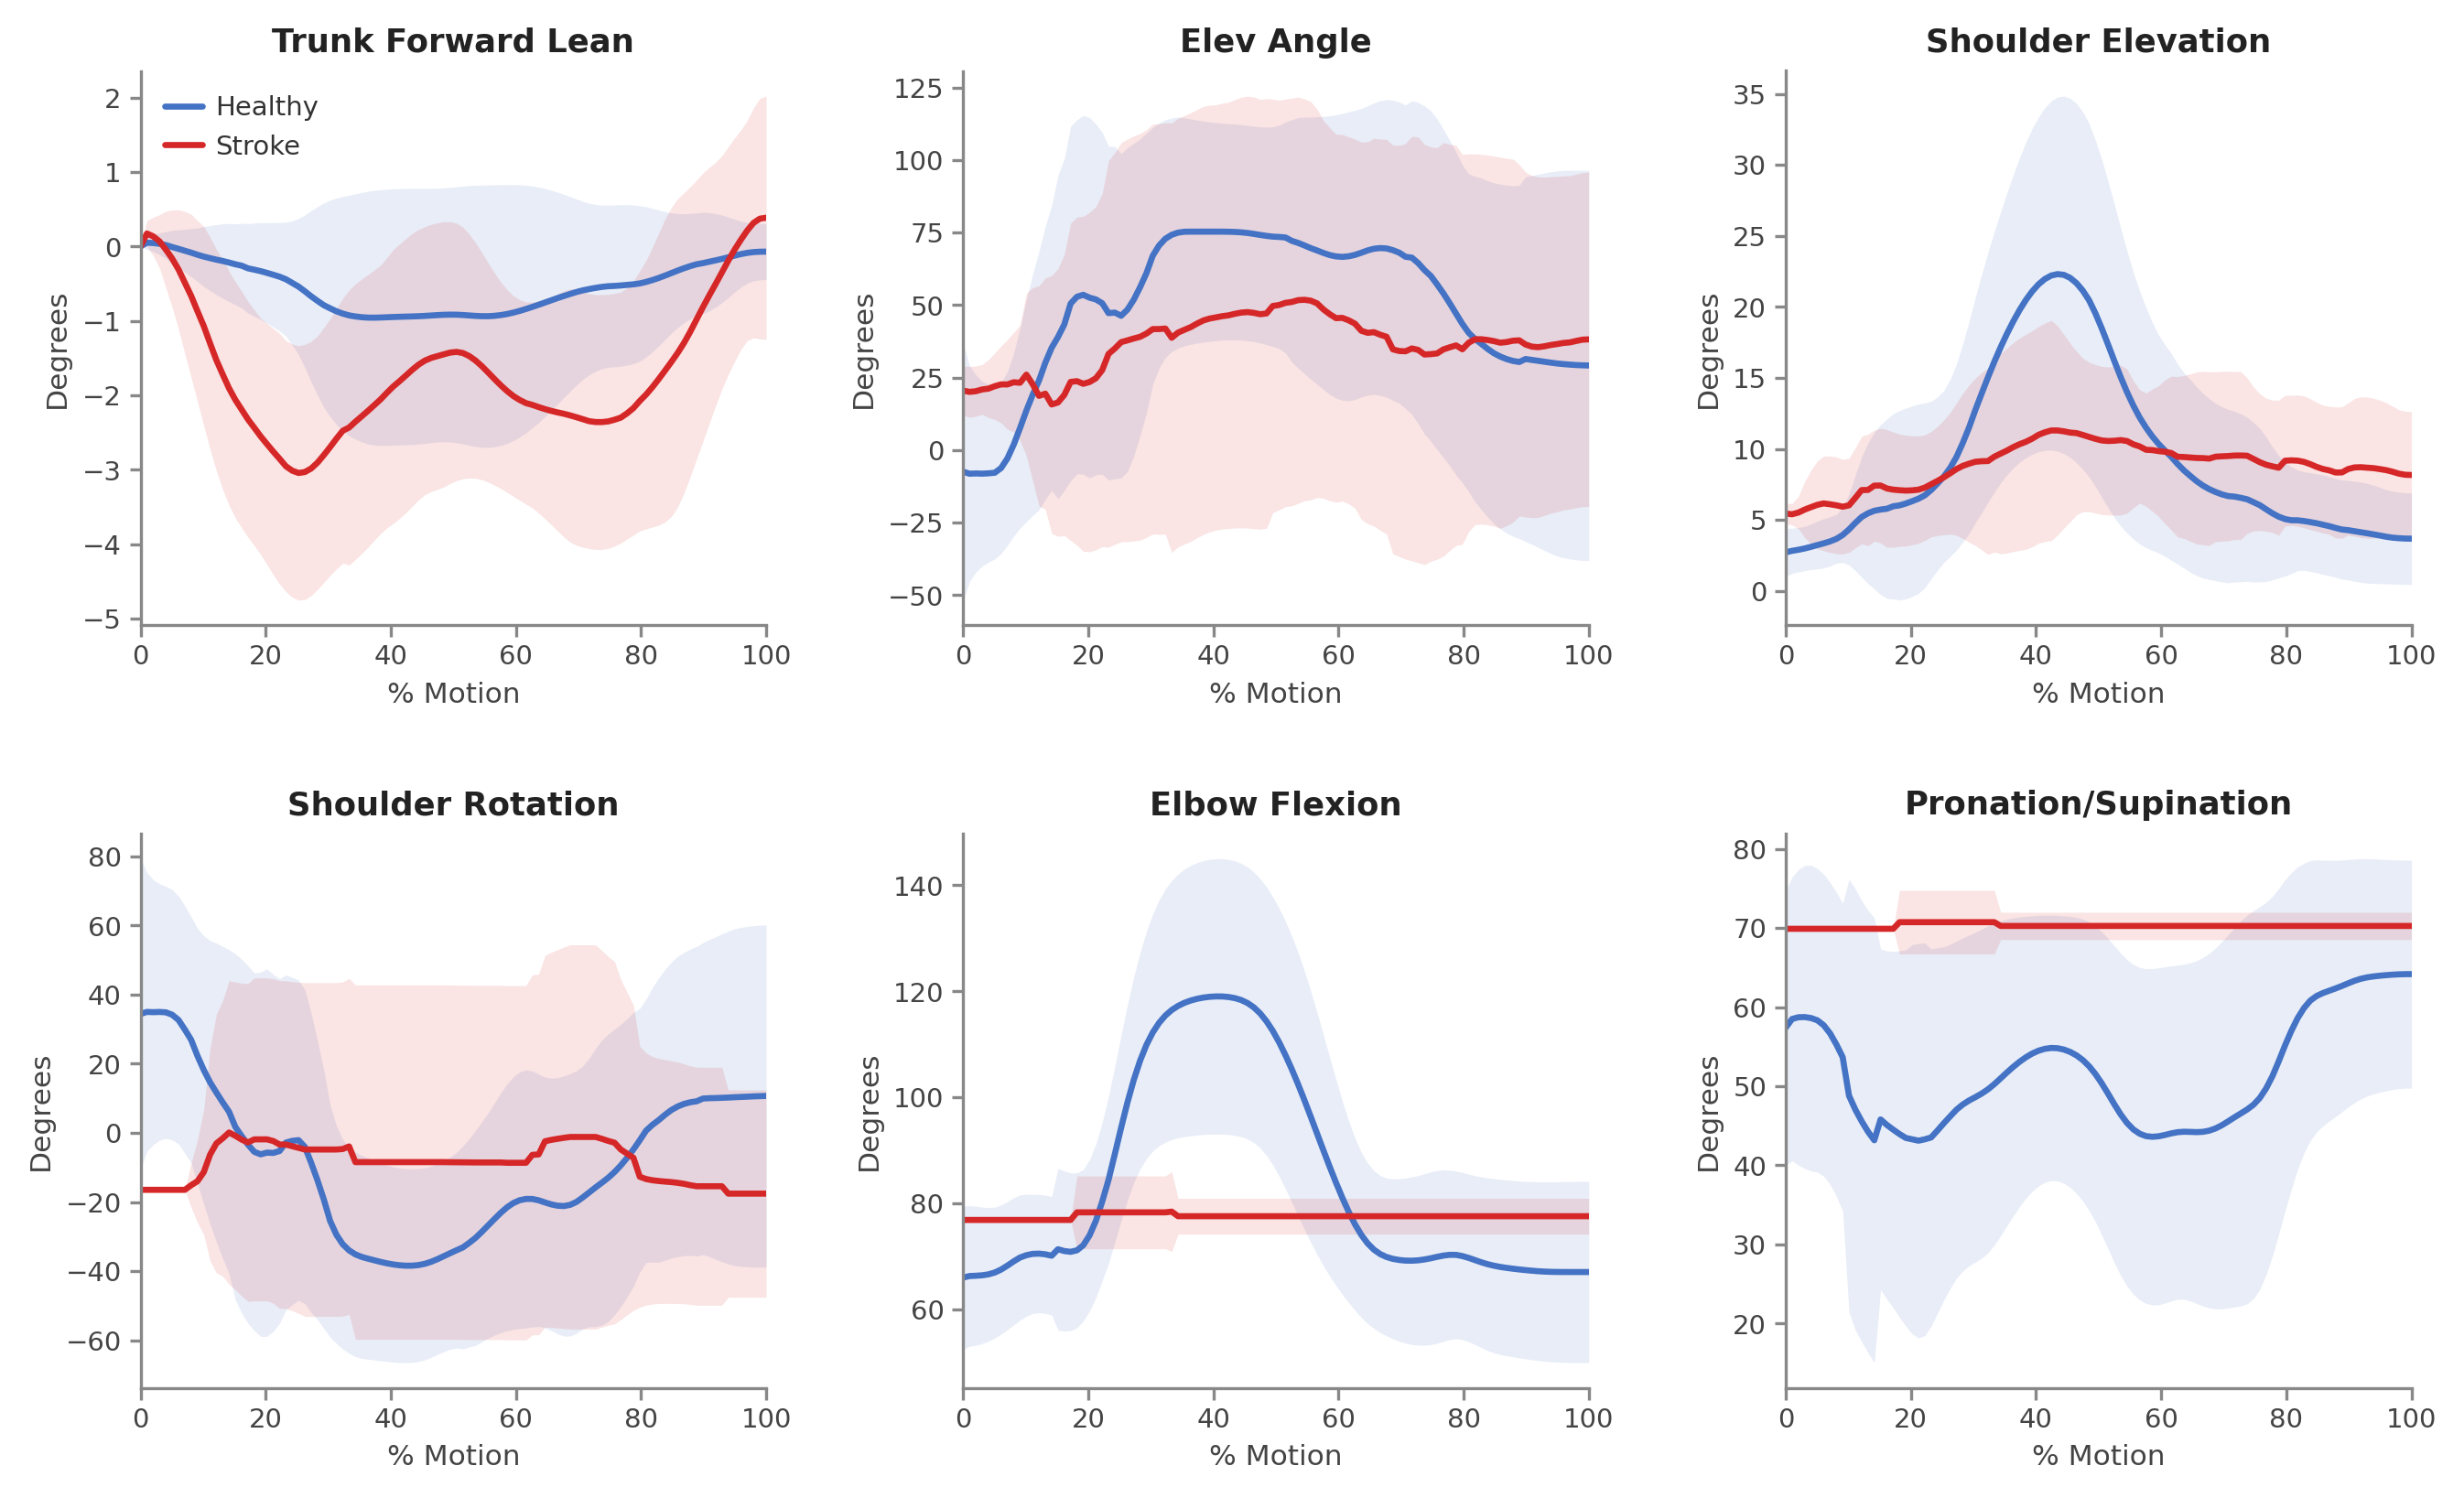
\includegraphics[width=\linewidth]{joint_trajectories_original.png}
    \caption{Group mean joint angles under Standard IK. The solver indiscriminately recruits the trunk, erasing expected clinical differences.}
    \label{fig:trajectories_original}
\end{figure}

\begin{figure}[!t]
    \centering
    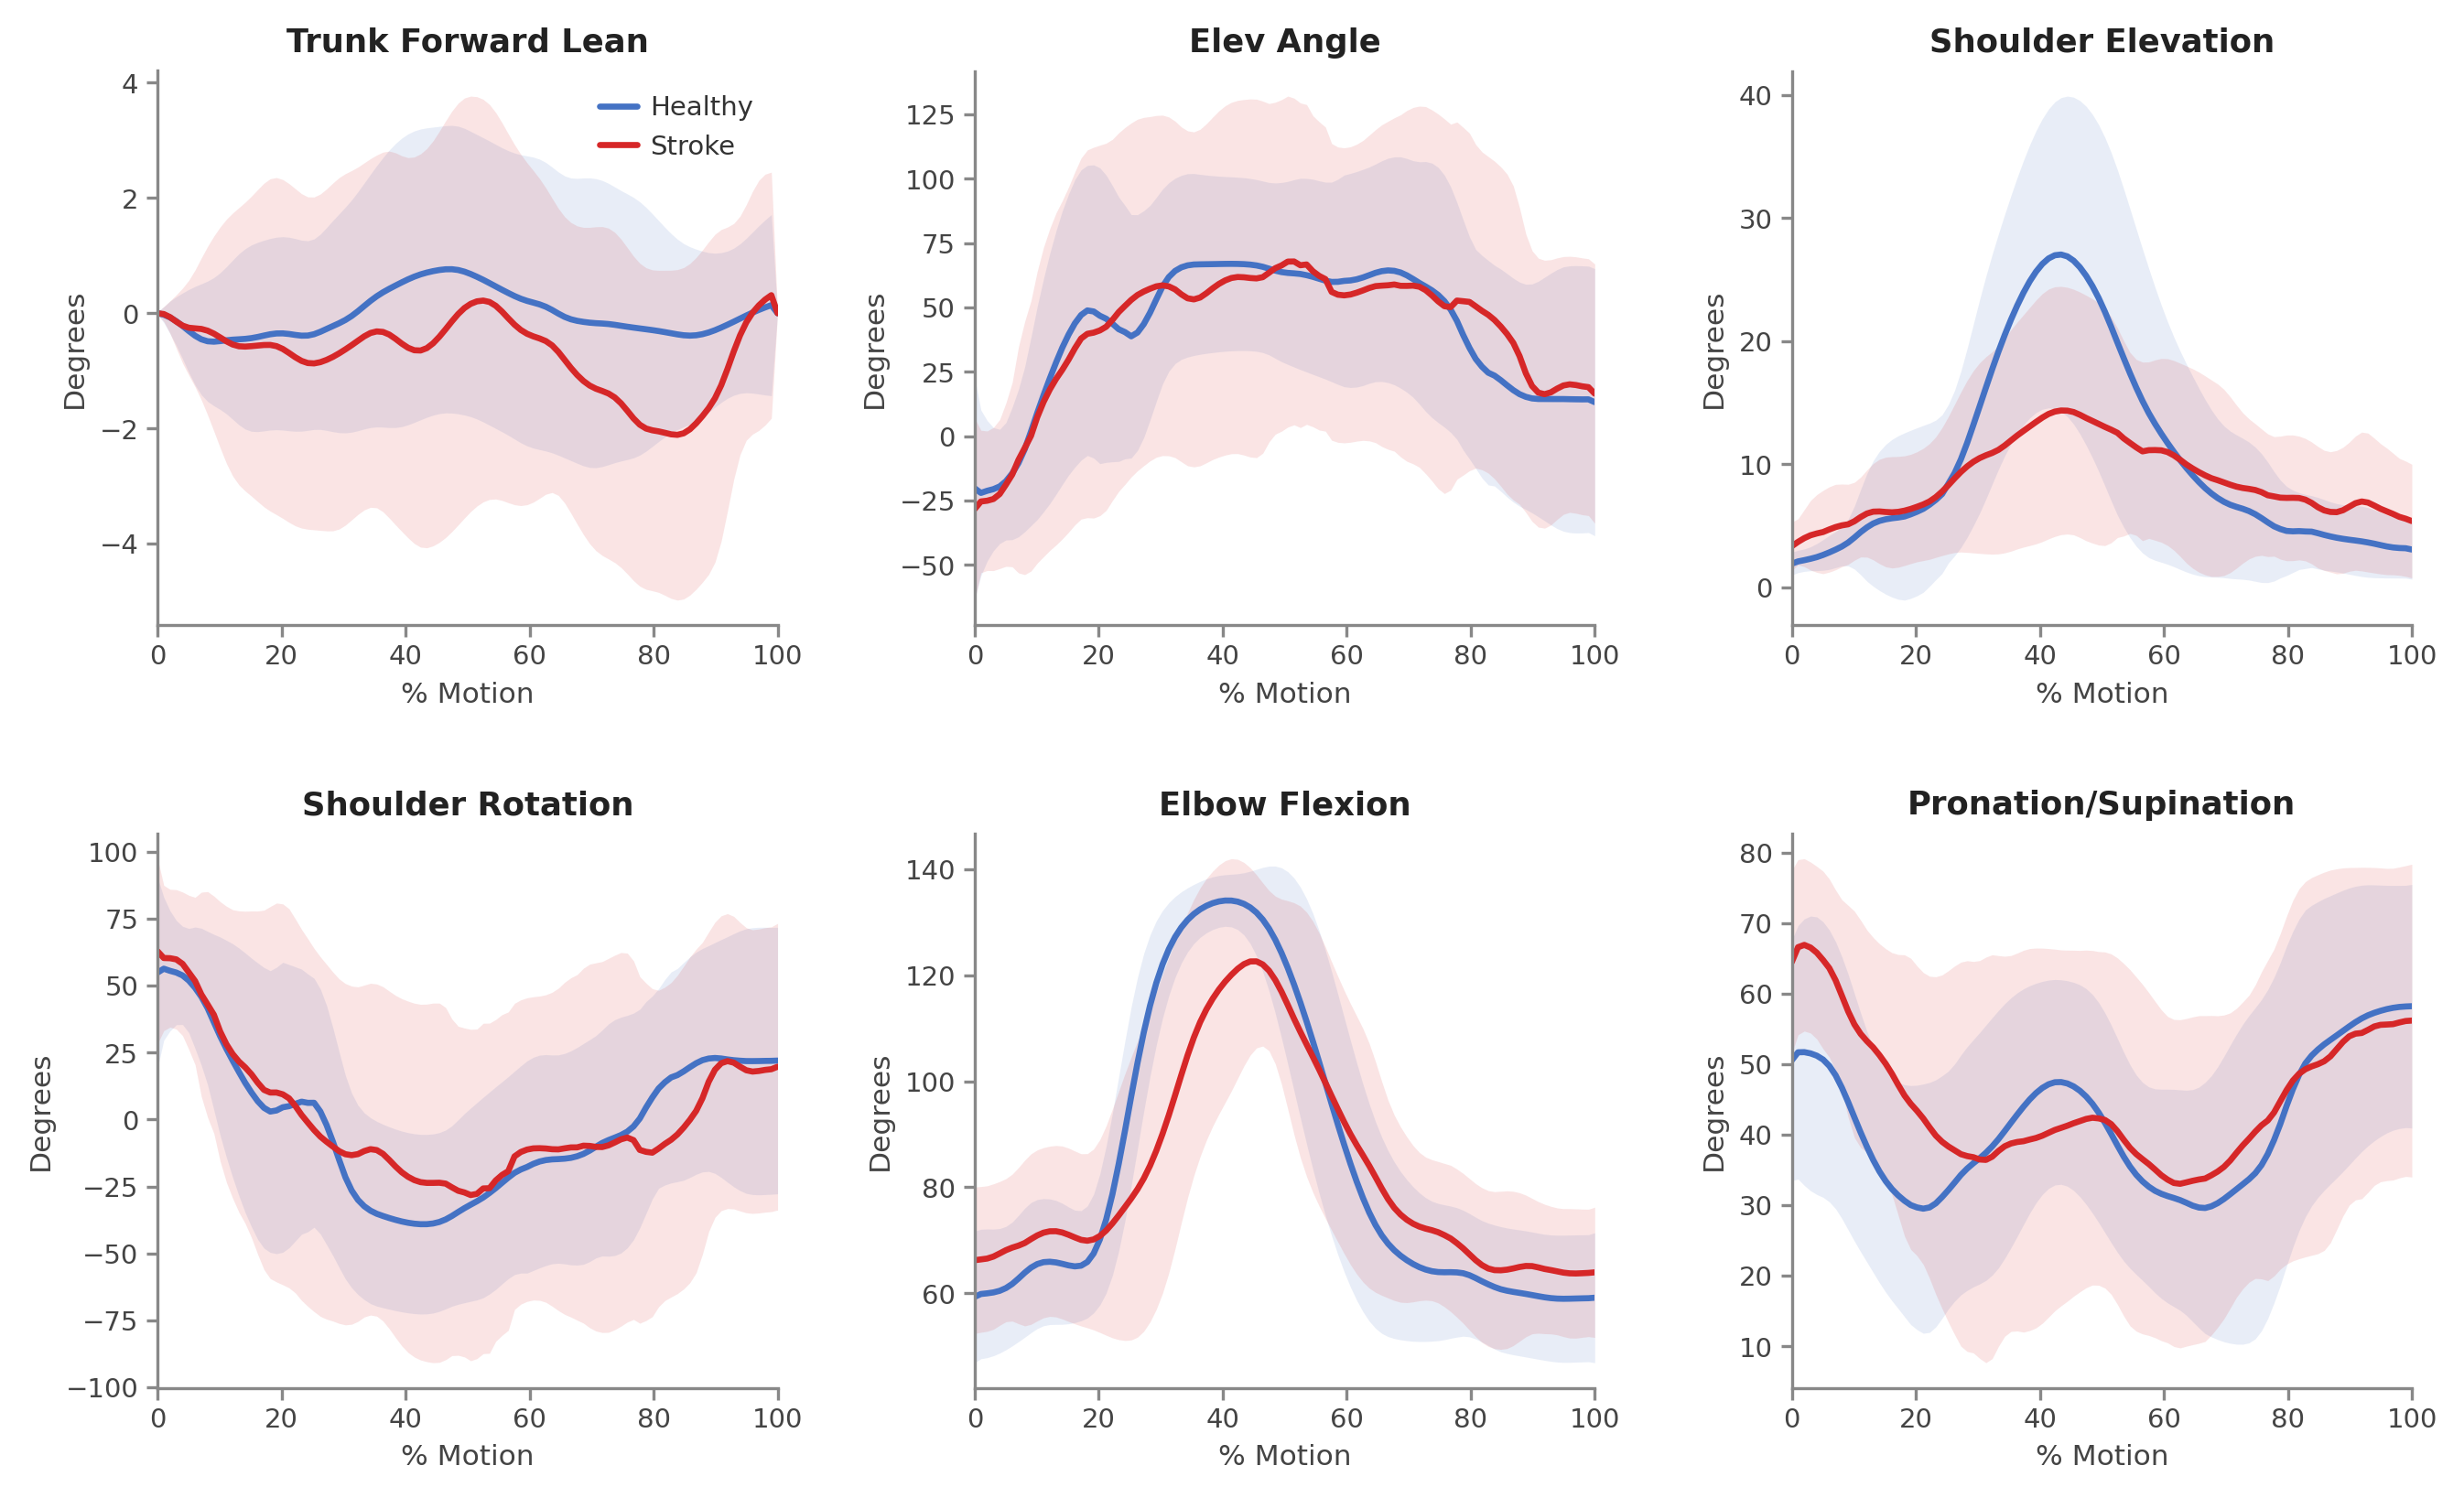
\includegraphics[width=\linewidth]{joint_trajectories_weighted.png}
    \caption{Group mean joint angles under the Two-Step Weighted IK. Trunk lean shows clear biological separation, and elevated pronation captures the flexor synergy.}
    \label{fig:trajectories_weighted}
\end{figure}

\begin{figure}[!t]
    \centering
    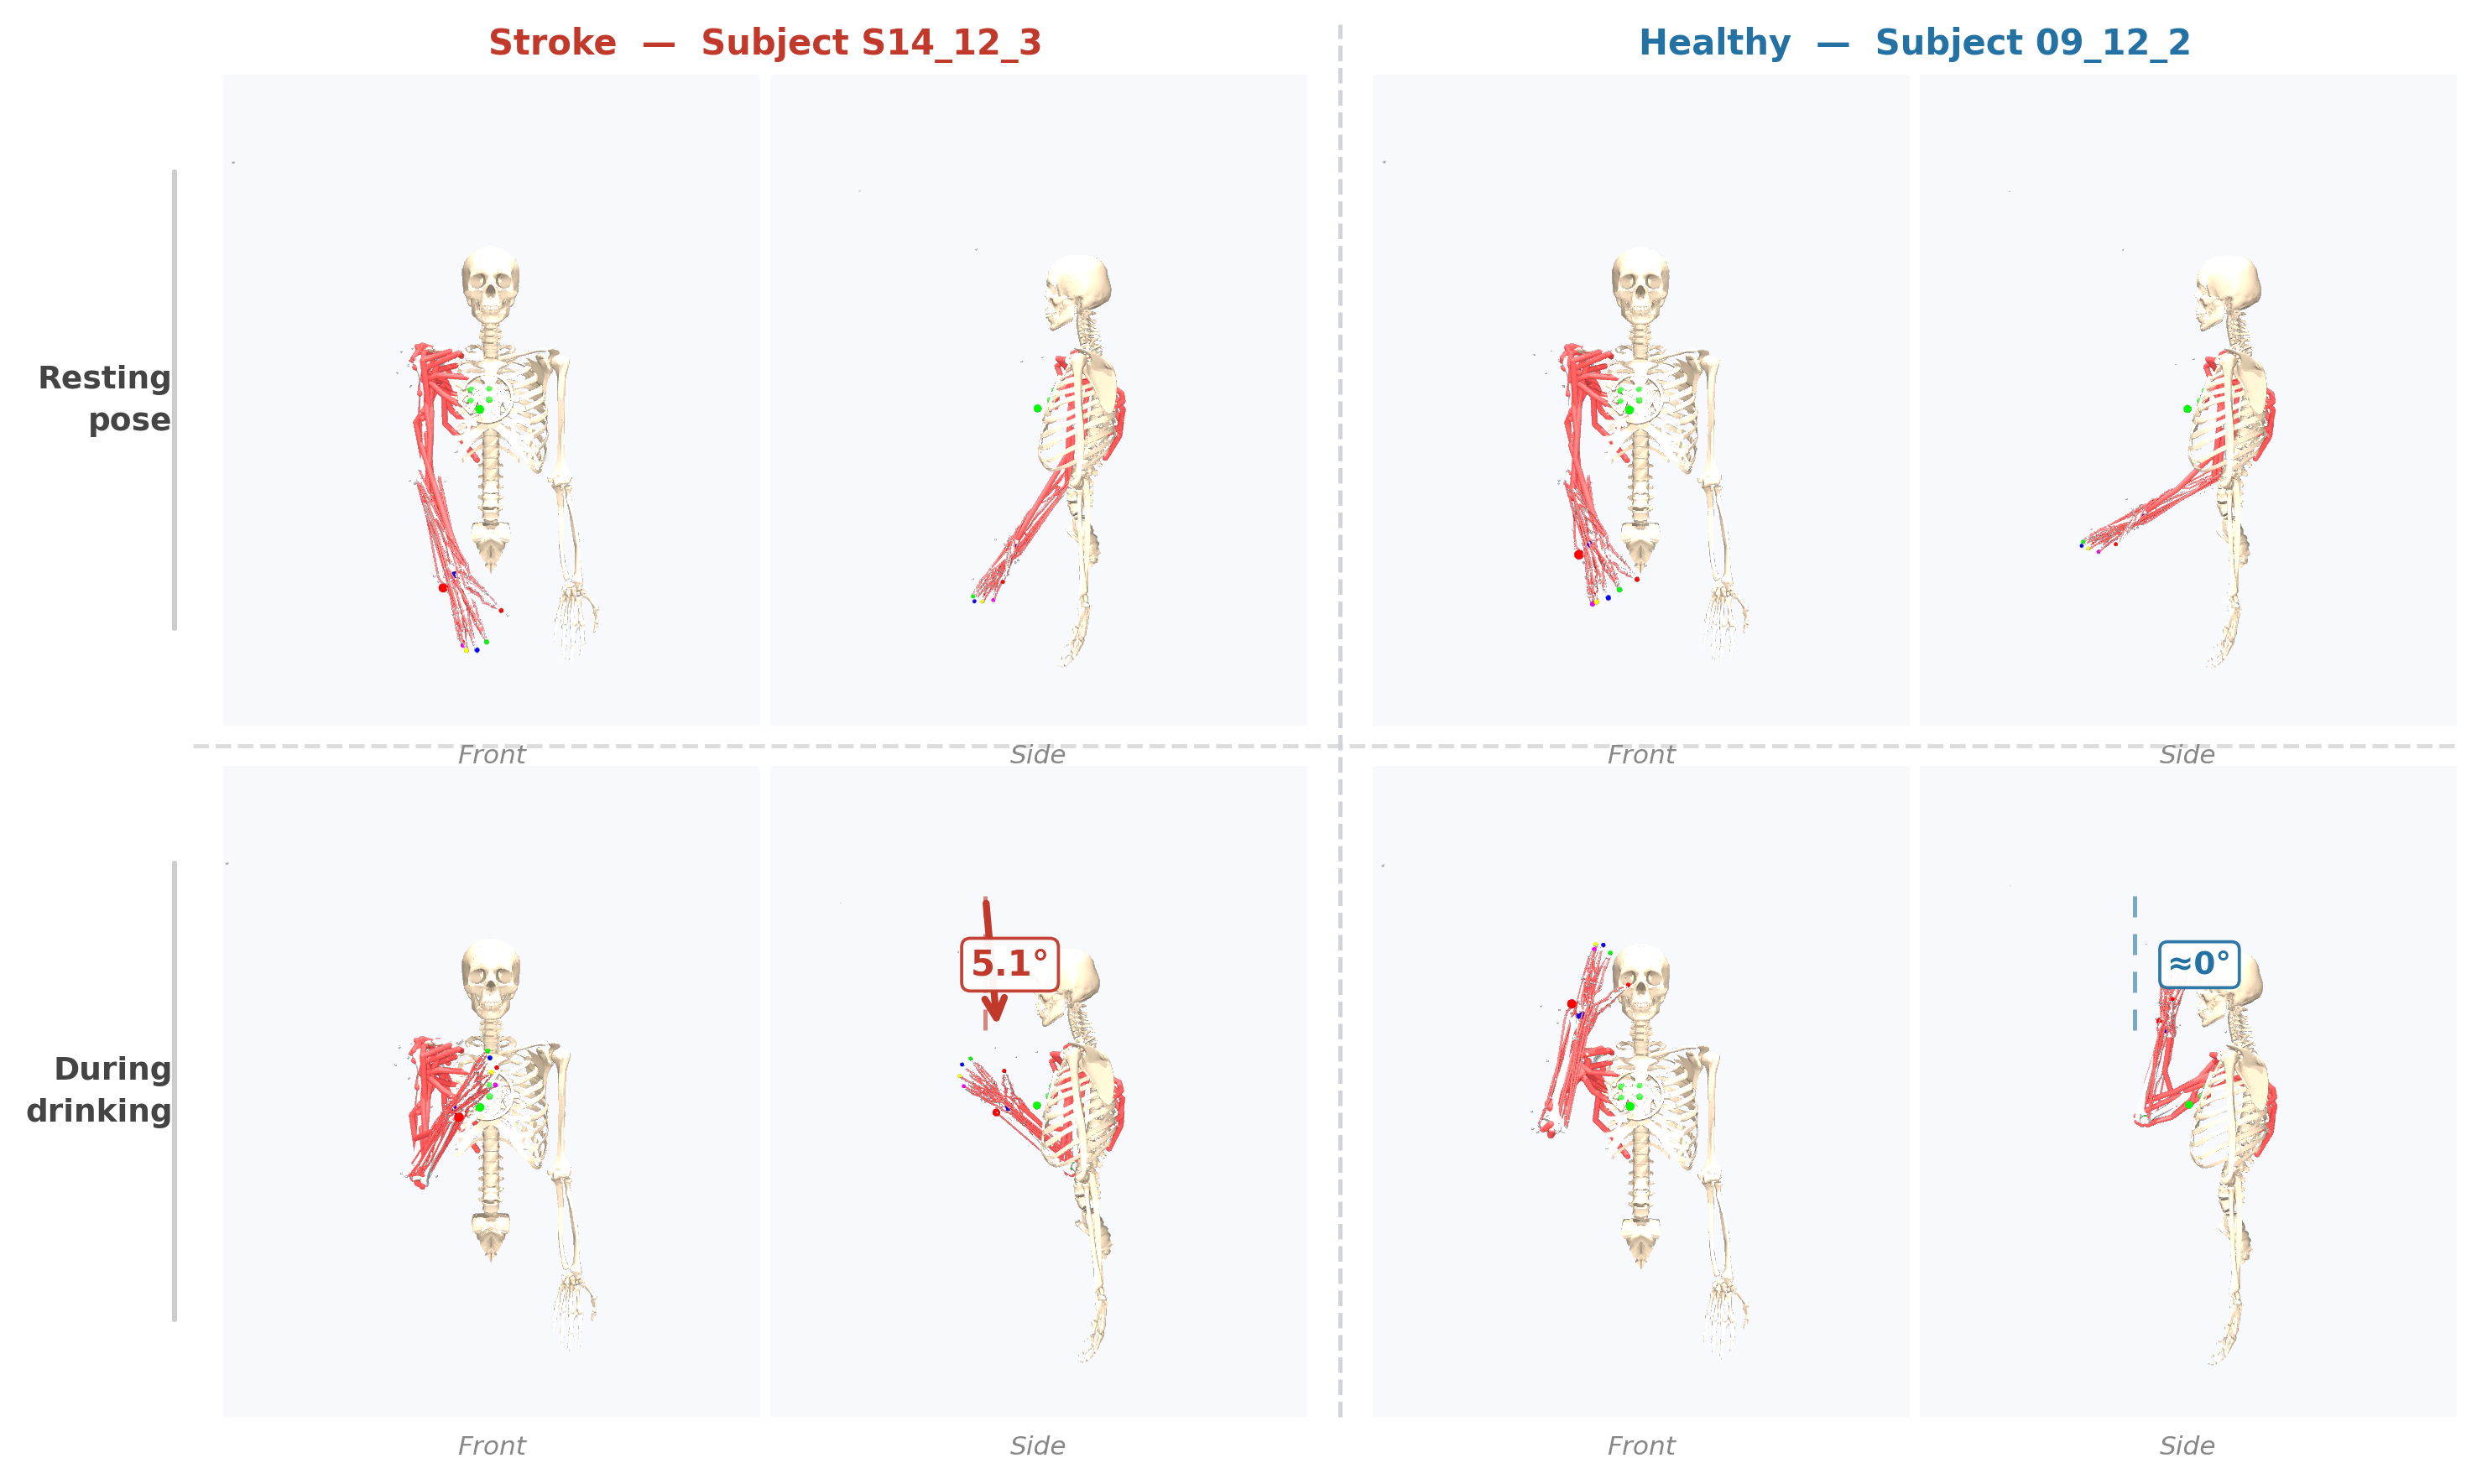
\includegraphics[width=\linewidth]{pose_comparison.png}
    \caption{Model postures at peak wrist height under the Two-Step Weighted IK. Left: stroke subject S14\_12\_3 (trunk lean $5.1^\circ$, shoulder elevation $4.7^\circ$). Right: healthy subject 09\_12\_2 (trunk lean $\approx 0^\circ$, shoulder elevation $55.5^\circ$). Resting (top) and drinking (bottom) frames are shown for each subject and view.}
    \label{fig:pose_comparison}
\end{figure}

\begin{table}[htbp]
  \centering
  \caption{Clinical Metrics (mean $\pm$ SD of per-subject peak values). Wtd.\ IK column reflects Two-Step Weighted IK results.}
  \label{tab:clinical_metrics}
  \vspace{0.5em}
  \resizebox{\linewidth}{!}{%
  \begin{tabular}{llcccc}
    \toprule
    \textbf{Metric} & \textbf{Group} & \textbf{Std. IK} & \textbf{Wtd. IK (mean $\pm$ SD)} & \textbf{$\Delta$ (W $-$ S)} & \textbf{Expected} \\
    \midrule
    \multirow{2}{*}{Trunk Lean (°)} & Stroke  & 3.9 & $4.25 \pm 2.34$ & $+$0.4 & \multirow{2}{*}{S $>$ H} \\
                                    & Healthy & 2.3 & $3.13 \pm 2.33$ & $+$0.8 & \\
    \midrule
    \multirow{2}{*}{Pronation (°)} & Stroke  & 70.7 & $73.84 \pm 13.92$ & $+$3.1 & \multirow{2}{*}{S $>$ H} \\
                                   & Healthy & 69.8 & $66.08 \pm 12.63$ & $-$3.7 & \\
    \midrule
    \multirow{2}{*}{Shoulder Elv. (°)} & Stroke  & 15.5 & $19.56 \pm 9.63$  & $+$4.1 & \multirow{2}{*}{S $<$ H} \\
                                       & Healthy & 19.7 & $28.73 \pm 13.08$ & $+$9.0 & \\
    \midrule
    \multirow{2}{*}{Elbow ROM (°)} & Stroke  & —    & $72.69 \pm 16.02$ & —      & \multirow{2}{*}{S $<$ H} \\
                                   & Healthy & 27.4 & $81.50 \pm 8.94$  & $+$54.1 & \\
    \bottomrule
  \end{tabular}}
\end{table}

\begin{figure}[!t]
    \centering
    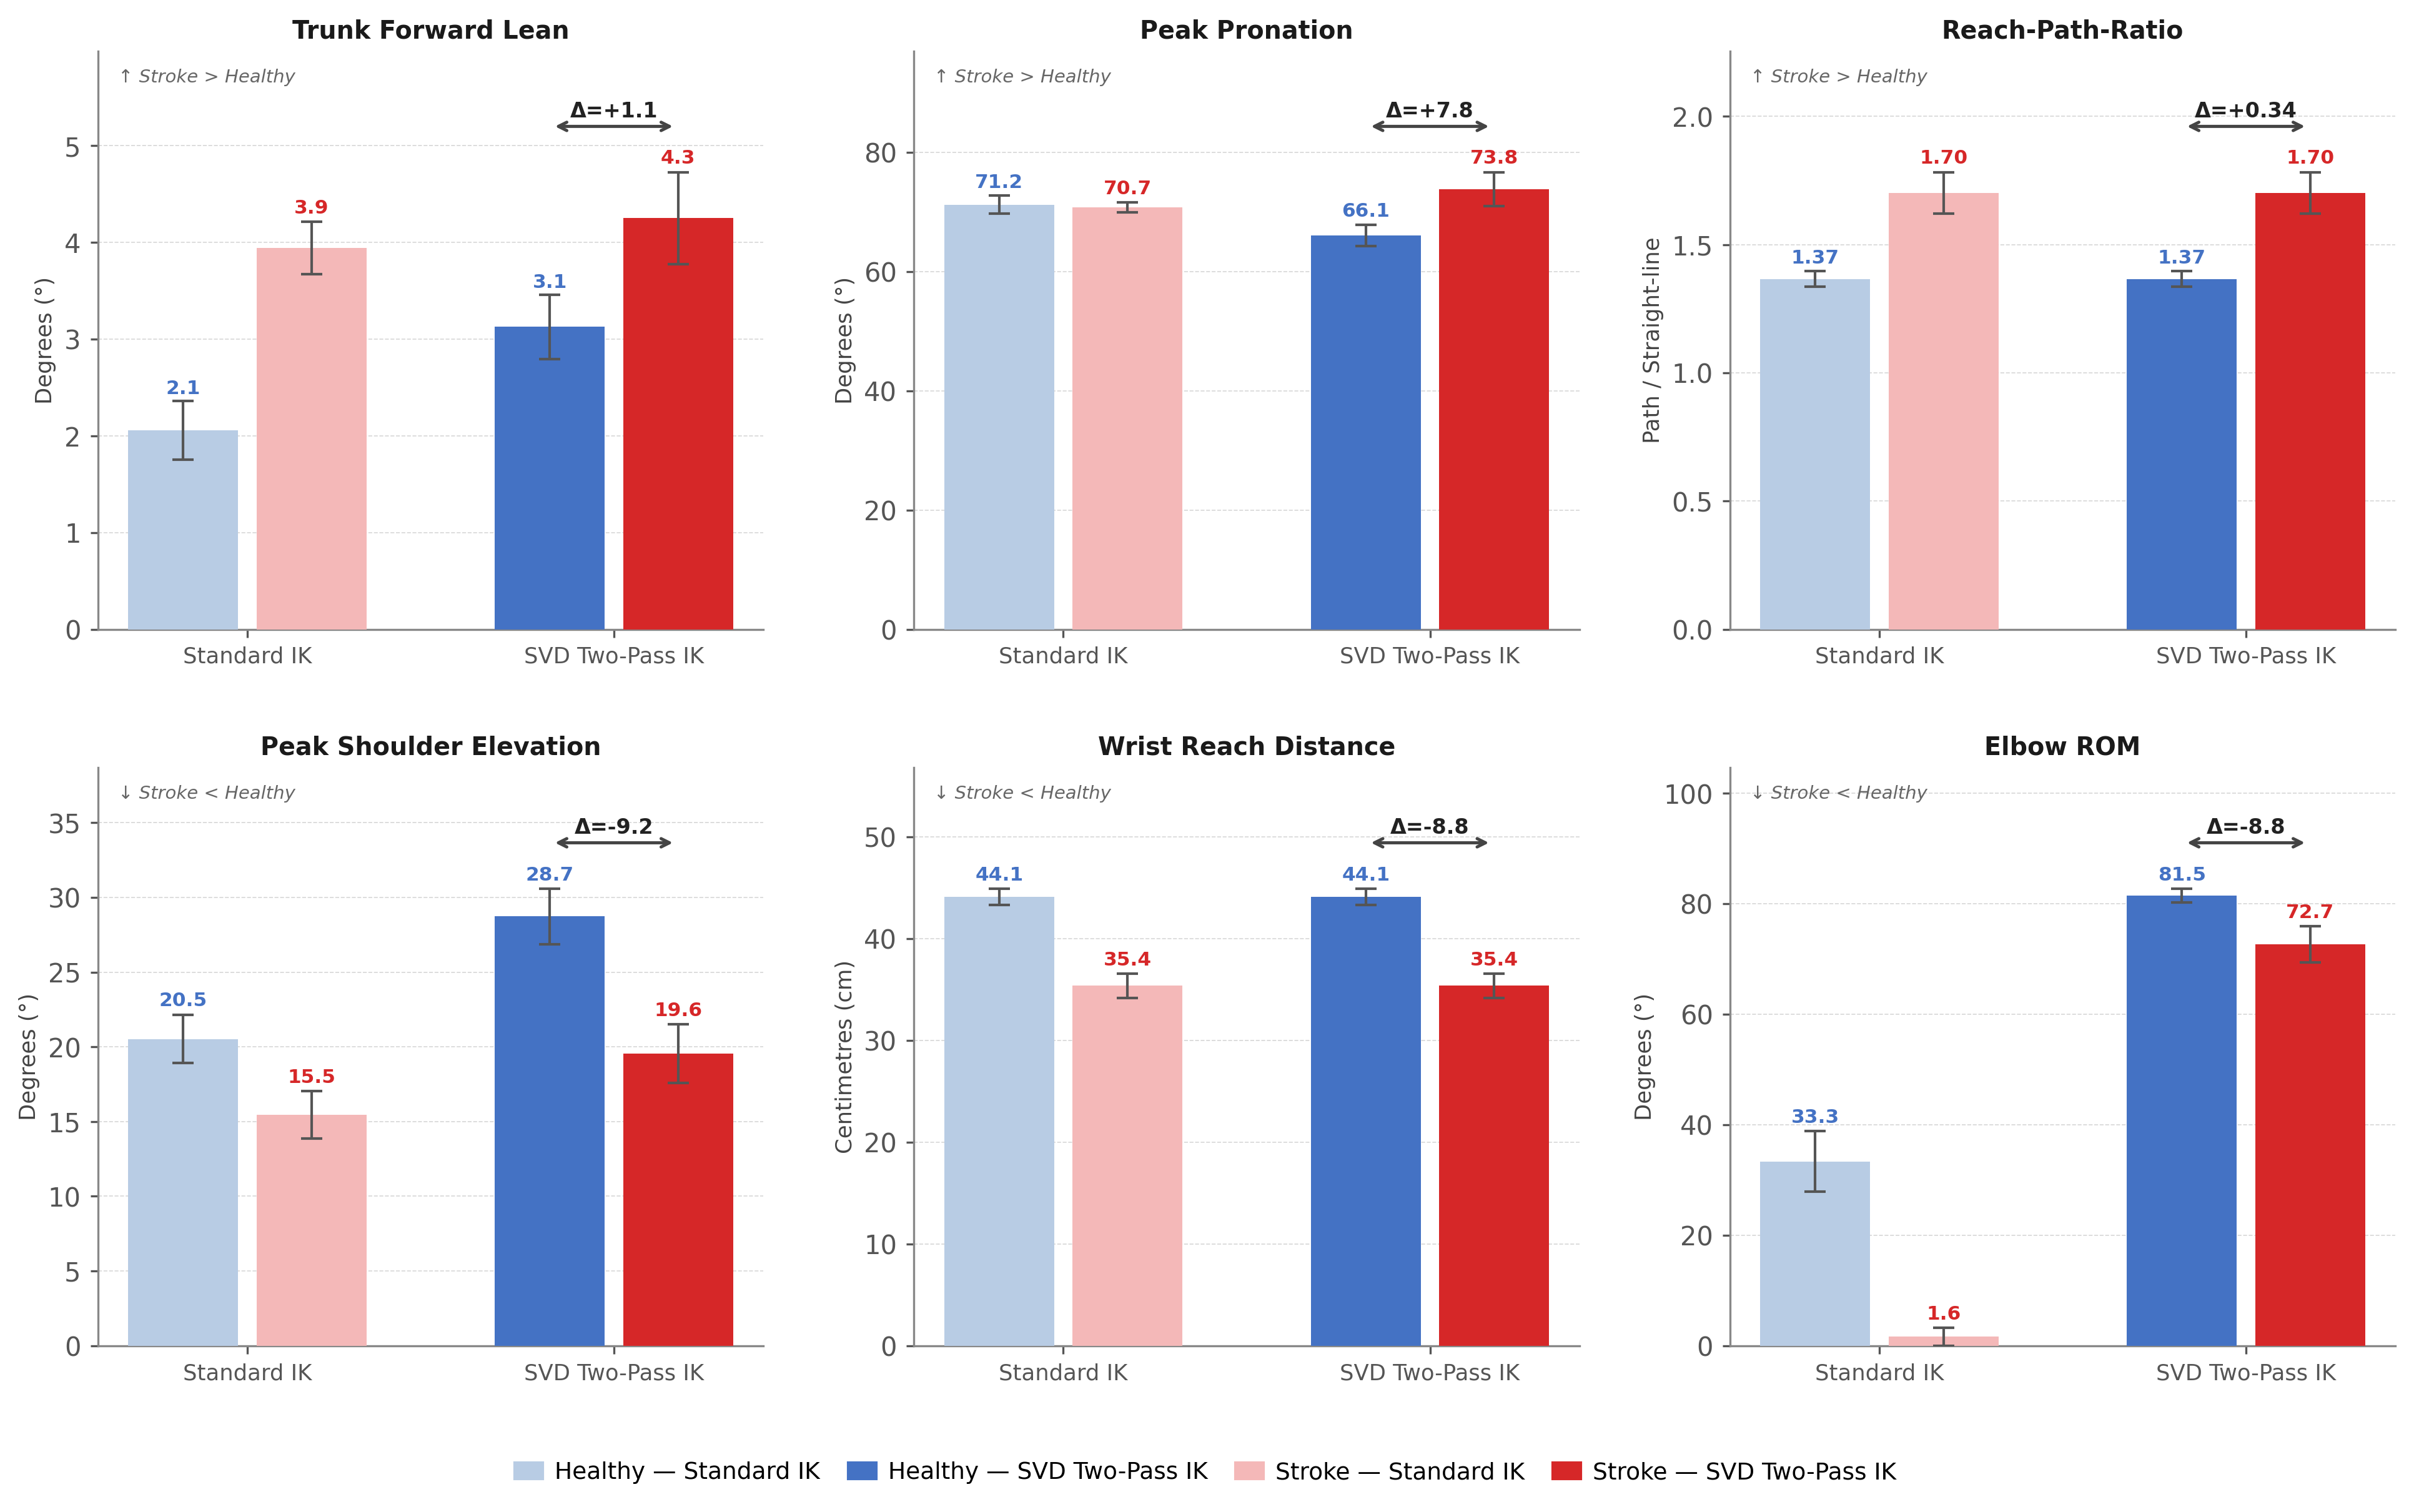
\includegraphics[width=\linewidth]{clinical_validation_results.png}
    \caption{Clinical validation results comparing metrics across IK pipelines. The Two-Step Weighted framework recovers physiologically valid kinematics, revealing clear inter-group separation in pronation, shoulder elevation, and elbow ROM.}
    \label{fig:clinical_validation}
\end{figure}

Furthermore, the 2-Tier Weighted Jacobian accurately preserved all other synergistic patterns expected in severe hemiparesis (Figure \ref{fig:distributions}):
\begin{itemize}
    \item \textbf{Flexor Synergy:} Stroke patients exhibited elevated peak pronation throughout the reach ($73.84 \pm 13.92$° vs.\ healthy $66.08 \pm 12.63$°; gap $+$7.7°).
    \item \textbf{Blunted Elevation:} Stroke shoulder elevation was restricted ($19.56 \pm 9.63$° vs.\ healthy $28.73 \pm 13.08$°; gap $-$9.1°).
    \item \textbf{Elbow ROM:} Functional elbow range was constrained in the stroke cohort ($72.69 \pm 16.02$° vs.\ healthy $81.50 \pm 8.94$°; gap $-$8.8°).
\end{itemize}
Figure \ref{fig:clinical_validation} summarises all six metrics side-by-side across both pipelines, directly illustrating the improvement in inter-group separation achieved by the Two-Step Weighted IK.


\begin{figure}[!t]
    \centering
    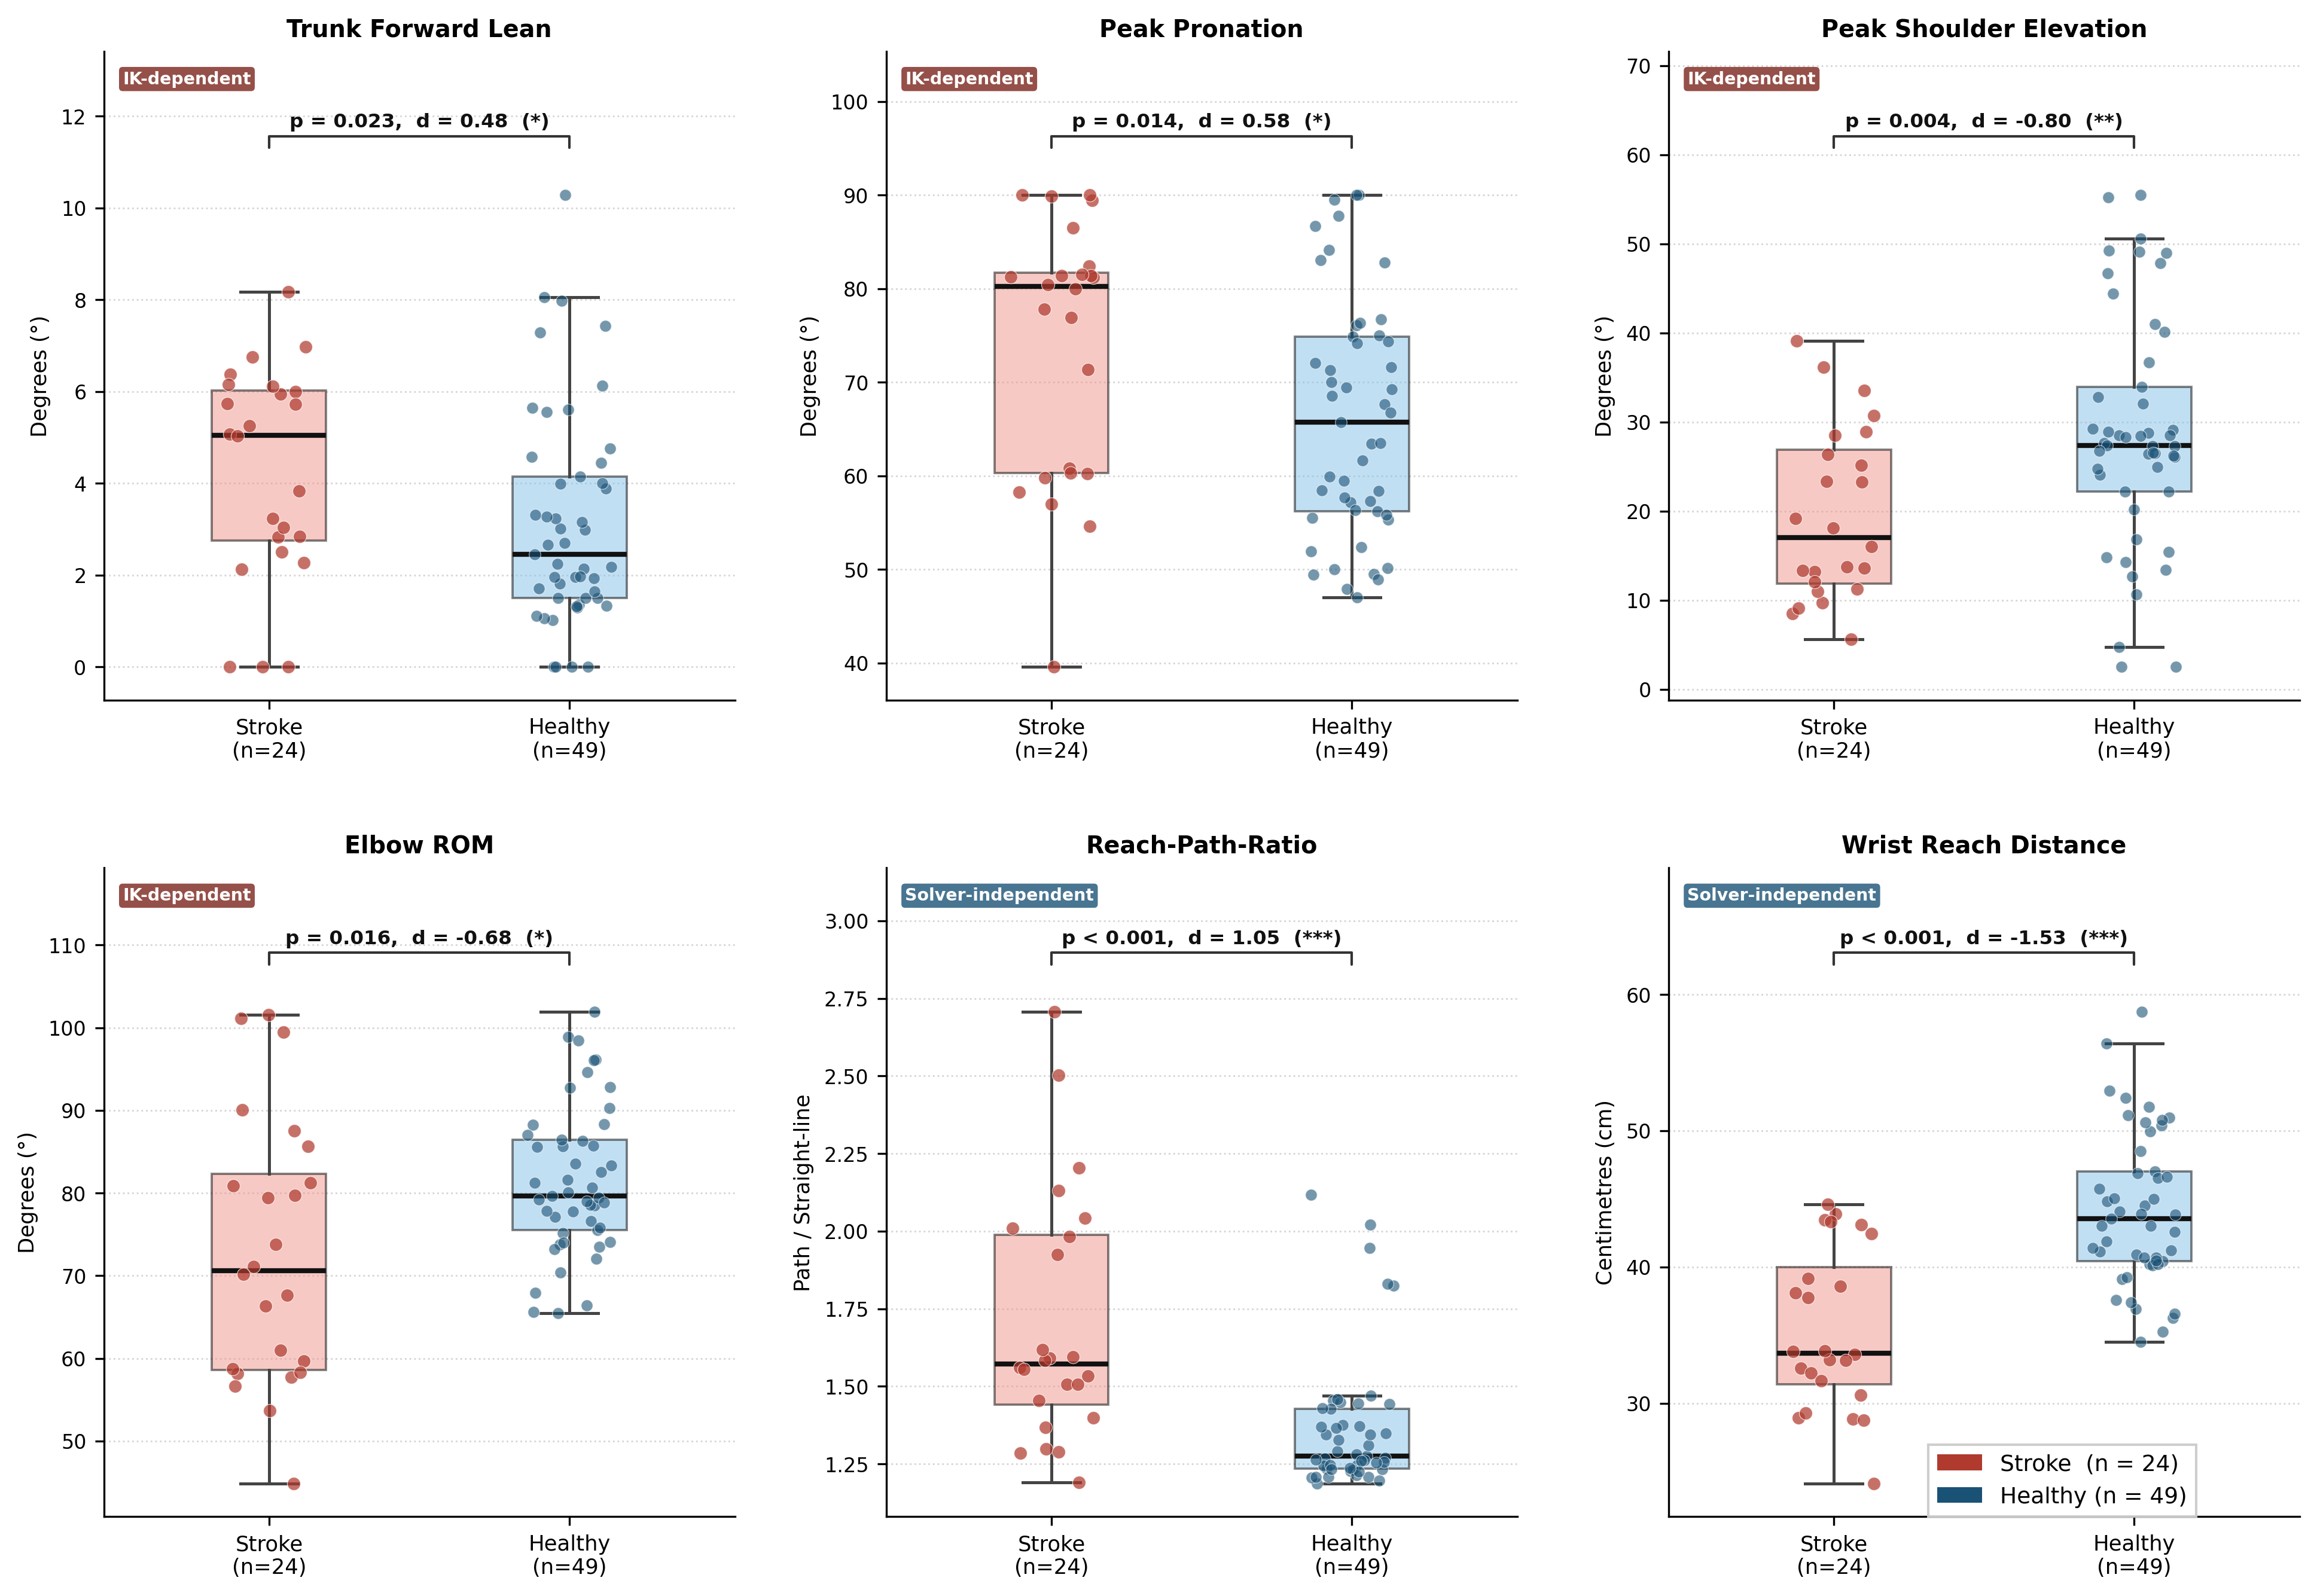
\includegraphics[width=\linewidth]{final_5_metric_distribution.png}
    \caption{Per-subject distributions for clinical metrics under Two-Step Weighted IK, demonstrating clear inter-group biological variance.}
    \label{fig:distributions}
\end{figure}

% ================================================================
\section{Discussion}
\label{sec:discussion}

Standard IK fails in sparse-marker clinical settings because it assumes geometric uniformity across patients. Tracking trunk movement through absolute marker position creates a depth-scaling problem that, without correction, causes the solver to collapse numerically with errors exceeding 300 mm. The core contribution of this work is demonstrating that both failure modes (geometric mismatch and unconstrained trunk recruitment) must be resolved together for clinically valid kinematics to emerge.

The proposed Two-Step Weighted IK framework resolves this gracefully. First, by using an orientation-based measurement for the trunk via SVD and segment-aware geometric scaling, we decouple the kinematic measurement from the physical depth of the subject. A 5° rotation of the marker plate yields 5° regardless of whether the patient has a deep or shallow chest cavity. 

Second, with the trunk prescribed to anatomical reality, pairing the arms with a 2-tier penalty weight ($w=0.20$ for the SC girdle) prevents the solver from hiding pathology in the upper limb. The framework has no knowledge of the patient's diagnosis, yet the pathological patterns emerge naturally from the data, with mean reconstruction errors of 44.97 mm (stroke) and 39.47 mm (healthy).

\subsection{Conclusion}
The Two-Step Weighted IK framework resolves two interacting failure modes that corrupt standard IK on sparse clinical marker sets: geometric depth mismatch and unconstrained trunk recruitment. By prescribing trunk lean from SVD plate orientation and penalising proximal shoulder-girdle joints, the pipeline stabilises reconstruction to clinically acceptable errors and recovers genuine pathological biomarkers in chronic stroke patients. The method requires only a standard sparse marker protocol, making it practical for routine clinical motion analysis.

\subsection{Limitations}
\label{sec:limitations}
The methodology is subject to specific limitations:
\begin{enumerate}
    \item \textbf{Narrow Cohort Variance:} The stroke cohort comprised only severe hemiparesis (FMA 16–20) performing a single sagittal drinking task, so sensitivity to moderate impairments remains untested. The framework's solver stability is general, but the specific biomarker thresholds reported here may not apply to mild stroke or other neurological conditions.
    \item \textbf{Trunk Measurement Dependency:} The SVD trunk angle depends on the chest plate being worn consistently. Plate slippage, repositioning between trials, or axial twist will introduce systematic error into the prescribed trunk value. A per-session baseline recalibration is assumed but not explicitly enforced.
    \item \textbf{Absence of Neuromuscular Validation:} While grounded in the CNS force-reserve principle, the sternoclavicular penalty weight ($w = 0.20$) is an empirically derived kinematic approximation. Although the dataset includes electromyography (EMG) recordings, cross-validating these weights against actual muscle activation was beyond the scope of this study. Future work incorporating EMG would further strengthen the biological validity of this cost hierarchy.
    \item \textbf{Rigid Model Geometry:} Fixing all nine mathematical correction joints at zero enforces an idealised skeletal geometry. While necessary to prevent anatomically impossible poses, this approach omits natural micro-translations within the shoulder complex (e.g., subtle scapular gliding or joint play). This rigidity is likely a contributing factor to the residual IK reconstruction errors observed, as the model cannot fully conform to each subject's true skeletal configuration. Though the primary clinical biomarkers are unlikely to be materially affected, minor systematic offsets in absolute joint angle estimates should be expected.
\end{enumerate}

% ================================================================
\section*{Ethics Statement}
This study used the publicly available, fully anonymised U-Limb motion capture dataset \cite{averta2021ulimb}. No additional ethical approval was required.

\section*{Funding}
This research received no specific grant from any funding agency in the public, commercial, or not-for-profit sectors.


\section*{Data Availability}
The code and processed data supporting the findings of this study are available from the corresponding author upon reasonable request.

\section*{Conflict of Interest}
The authors declare no conflict of interest.

\section*{Acknowledgements}
The authors would like to thank the creators of the U-Limb dataset and the MyoSuite framework for making their data and tools publicly available. No other contributors are to be acknowledged. This research received no external funding, and no funding was received for writing assistance.

% ================================================================
\section*{Declaration of generative AI and AI-assisted technologies in the manuscript preparation process}
During the preparation of this work the author(s) used Claude Opus 4.7 (Anthropic) in order to assist with structural organisation, manuscript framing, and refining the phrasing of author-written sentences for clarity. After using this tool/service, the author(s) reviewed and edited the content as needed and take(s) full responsibility for the content of the published article.

\bibliographystyle{elsarticle-harv}
\bibliography{references}

\end{document}